\documentclass[review]{elsarticle}

\usepackage{amsmath,amssymb,amsthm}
\usepackage{booktabs}
\usepackage{graphicx}
\usepackage{siunitx}
\sisetup{detect-all}
\usepackage[colorlinks,linkcolor=blue,citecolor=blue,urlcolor=blue]{hyperref}
\usepackage{xcolor}

\newtheorem{proposition}{Proposition}
\newtheorem{remark}{Remark}
\setlength{\emergencystretch}{3em}

\newcommand{\icast}{\boldsymbol{i}_{c,\ast}}
\newcommand{\ic}{\boldsymbol{i}_c}
\newcommand{\ip}{\boldsymbol{i}_p}
\newcommand{\psic}{\boldsymbol{\psi}_c}
\newcommand{\psip}{\boldsymbol{\psi}_p}
\newcommand{\Cmat}{\boldsymbol{C}}
\newcommand{\Wco}{W'}
\newcommand{\todonum}[1]{\textcolor{red}{[#1]}}

\journal{Advanced Engineering Informatics}

\begin{document}

\begin{frontmatter}

\title{Coverage-controlled learning of connection-invariant magnetic
surrogates for reconfigurable electric machines}

\author[inst1]{\todonum{Author Name}}
\affiliation[inst1]{organization={\todonum{Affiliation}},
            city={\todonum{City}},
            country={\todonum{Country}}}

\begin{abstract}
Reconfigurable windings (series--parallel, star--delta, taps, open-end)
extend the speed range and part-load efficiency of electric machines, yet
every candidate connection is still evaluated with its own dedicated
finite-element (FE) model or flux-map table, leaving the combinatorial
connection space unexplorable at design time. We treat a winding
connection as what it physically is: linear constraints on the coil
currents, $\ic=\Cmat\ip$. Because the magnetic co-energy is
connection-invariant, a single \emph{connection-invariant surrogate},
trained once on coil-level FE data, can be queried on unseen connections;
its zero-shot reliability is controlled by current-space coverage.
We formalise this generalisation problem with a qualitative coverage bound
for the training current distribution (rank correlation $0.82$ over seven
hold-outs); instantiate the surrogate with a structured co-energy network
whose reciprocity and torque--flux consistency hold by construction
($4.6\times10^{-4}$ vs $0.22$ for a black-box MLP); and release a
seven-connection, three-tier benchmark on a 12-slot/4-pole machine. The
benchmark yields two data-collection principles: what \emph{kind} of
current patterns is covered dominates how many samples exist. Magnitude-
random patterns (48 groups) reduce an unbalanced hold-out from flux nRMSE
$1.00$ to $0.11$ but leave an open-phase connection at $1.38$; 24
\emph{phase}-random groups---a quarter of the FE cost---bring it to
$0.07$ and the star--delta hold-out from $0.27$ to $0.07$; both
principles replicate on a second machine. A
monotonicity-constrained architecture fails outright ($\ge0.28$
everywhere): the joint co-energy is not convex. Finally, on the official
WLTC class-1 cycle with four identical 12-slot/4-pole wheel motors and a
400-V SiC drive, the only fully feasible fixed connection is 4P; a
dynamic-programming schedule uses $458.3$\,Wh ($40.1$\,Wh/km), a
$3.1\,\%$ saving. Raising the bus above $\approx$700\,V makes fixed delta
fully feasible and reduces the scheduling gain to $0.4$--$0.6\,\%$. An
independent FEMM cross-check reproduces the inductance shape after a
$1.13\times$ normalisation and saturated torque within $1.2\,\%$, but PM
fundamental amplitudes differ by $42\,\%$. At 36 synchronous points, the
never-trained 3S1P connection transfers torque with correlation $0.79$,
while the out-of-support tap50 torque screen remains unreliable. We therefore present reconfiguration as a
conditional design option rather than a universal efficiency gain.
\end{abstract}

\begin{keyword}
winding reconfiguration \sep magnetic co-energy \sep surrogate modelling \sep
zero-shot generalisation \sep physics-informed neural networks \sep
drive-cycle optimisation
\end{keyword}

\end{frontmatter}

\section{Introduction}
\label{sec:intro}

\subsection{Motivation}

Reconfigurable machine windings---series--parallel changeover, star--delta
switching, mid-winding taps, open-end windings and post-fault
reconfiguration---trade voltage class against current class at run time.
Recent reviews \cite{Best2025Access, RSER2025} report torque and
power-density gains of 40--80\,\%, machine
loss reductions of 30--60\,\%, and inverter current reductions above 40\,\% on
a production passenger car \cite{Best2025Access}. The enabling physics has
been demonstrated repeatedly: series connection multiplies the back-EMF and
suits low-speed high-torque operation, while parallel connection divides it
and extends the constant-power speed range \cite{Shin2024WEVJ,
TMAG2012Changeover}.

What has \emph{not} kept pace is the modelling machinery. Every published
study evaluates two to four hand-picked connections, each with its own FE
model or its own $dq$ flux-map table. For a machine with four coil groups per
phase the discrete connection space already contains hundreds of meaningful
entries (series--parallel groupings, taps, star/delta, open-winding, degraded
states), and each FE campaign takes hours to days. The 2025 review is
explicit: the field lacks (i)~early-stage design methods that compare
connections systematically, (ii)~drive-cycle-level switching strategies, and
(iii)~system-level loss accounting that includes the changeover circuit
\cite{Best2025Access}. Concurrently, the transient-control side of the
problem has been pushed to near-optimal territory---recent deadbeat
predictive control achieves $5\,\mu$s seamless changeover with no torque
interruption \cite{Guo2026Electronics, TPEL2026Seamless,
JESTPE2026Seamless}---so the bottleneck has decisively shifted from
``how to switch'' to ``what to switch to, and when''.

\subsection{Related work and the gap}

\paragraph{Analytic connection selection.}
Normalised characteristic-current criteria map connection families onto a
single $\hat{I}_{ch}$--$\xi$ plane and give closed-form decision thresholds
\cite{Energies2026Ich}. These are valuable screening tools, but they are derived
under the assumptions of linearity, negligible cross-saturation and
negligible losses; the same paper lists
drive-cycle optimisation and switching transients as open problems. Analytic
criteria cannot exploit the nonlinear multi-coil physics that FE already
provides.

\paragraph{Learned magnetic surrogates.}
Neural mappings of flux linkage and torque are standard for fixed windings:
ANN torque surrogates \cite{Access2020ANNReview}, physics-informed
networks \cite{Raissi2019PINN} including PINN-parameterised PMSM
fields \cite{TEC2025PINN}, POD/SVR fast surrogates \cite{Arxiv2024POD},
Fourier neural operators \cite{Li2021FNO} for FE acceleration
\cite{DETC2025FNO}, and
data-efficient \emph{gradient networks} that learn the magnetic
co-energy/flux-linkage map with reciprocity and energy conservation enforced
by the architecture \cite{Li2026GradNet}. All of these operate on the
$d$--$q$ plane of \emph{one} fixed winding; changing the connection changes
the input dimension itself, so the model must be retrained. None of them
addresses topology generalisation.

\paragraph{Winding-level reconfiguration studies.}
Series--parallel changeover hardware and control are mature
\cite{Shin2024WEVJ, TIA2024MechChangeover, IPEC2014}; open-end
and multi-mode drives select the best mode pointwise \cite{Cha2024Math};
three-speed tapped IPMSMs \cite{TIE2026Tap} and reconfigurable SRM windings
\cite{TTE2025SRM} extend the principle. Mode selection, however, is either a
fixed speed threshold or a per-point greedy choice; no study optimises the
\emph{sequence} of modes over a drive cycle with changeover losses and dwell
constraints, and losses of the changeover circuit itself are usually ignored
\cite{Best2025Access}.

\paragraph{The gap.}
Three communities hold one piece each: connection physics (electrical
machines), structure-enforcing ML (co-energy/gradient networks), and
scheduling (energy management). What is missing is the bridge:
\emph{a single magnetic model that can be queried across candidate
connections, with coverage characterising when transfer is reliable}. If the
connection is only a linear constraint on coil currents, such a model turns
connection exploration from ``one FE campaign per connection'' into ``one
training run plus a matrix product'', and makes drive-cycle co-design of
topology and schedule computationally trivial.

\subsection{Contributions}

\begin{enumerate}
\item \textbf{Problem formulation and theory
(\S\ref{sec:formulation}).} We cast winding reconfiguration as constrained
regression in coil-current space, prove that the co-energy and its derivatives
are connection-invariant (Prop.~\ref{prop:invariance}), and give a
qualitative bound for zero-shot transfer to unseen connections governed by the
coverage distance of the training current distribution
(Prop.~\ref{prop:bound}). The qualitative implication is consistent with
the experiments: connections whose current vectors lie inside the training support
transfer at in-distribution accuracy, while support-extrapolating connections
fail until the support is extended; the coverage distance correlates with
zero-shot error at rank $\rho=0.82$ over seven hold-outs, with
informative misalignments that delimit when the screen applies.
\item \textbf{Connection-invariant structured co-energy network
(\S\ref{sec:method}).} A scalar co-energy head with a
Fourier-parameterised, PSD-seeded inductance matrix, harmonic PM flux and a
zero-initialised residual MLP. Reciprocity, energy conservation and
torque--flux consistency hold by construction to autograd precision
($4.6\times10^{-4}$ measured), versus $0.22$ for a same-size MLP. The
structure is offered as a consistency option, not an accuracy winner: an
unstructured MLP remains more accurate on in-support hold-outs and on the
torque channel, and the benchmark quantifies this trade-off rather than
claiming dominance. We also
report an instructive negative result: a monotone (PSD-Jacobian,
input-convex-style \cite{Amos2017ICNN}) vector-field
parameterisation fails at all difficulties because the joint co-energy is not
convex in $(\ic,\theta)$.
\item \textbf{A stratified zero-shot benchmark with data-design principles
(\S\ref{sec:benchmark}--\ref{sec:results}).} Seven hold-out connections
across three difficulty tiers, 9{,}276 nonlinear FE samples (23{,}000+
including the drive-cycle pools), four model
families, and a reproducible split protocol. Two findings generalise beyond
this machine: (i)~48 magnitude-random current patterns rescue unbalanced
connections (nRMSE $1.00\!\to\!0.11$) where doubling standard-connection data
does not help; (ii)~phase-random patterns (a quarter of the magnitude family's FE cost) rescue
open-phase connections that magnitude patterns cannot ($1.38\!\to\!0.07$).
Coverage \emph{kind} dominates coverage \emph{amount}; both
principles replicate on a 6-slot/4-pole second machine.
\item \textbf{Drive-cycle stress test and zero-shot limits
(\S\ref{sec:drive}).} The surrogate
generates mode-conditioned loss maps in milliseconds; a dynamic program over
the official WLTC class-1 trace jointly selects connection and operating
point under voltage envelopes, current limits, minimum dwell and changeover
energy. In a current-matched four-motor calibration at 400\,V, only 4P can
complete the cycle as a fixed mode; the DP schedule saves about $3.1\,\%$.
At 700\,V and above, fixed delta becomes feasible and the gain collapses to
$0.4$--$0.6\,\%$. The benefit is therefore conditional on the voltage and
current envelope. The same
surrogate transfers torque to a never-trained 3S1P connection
(correlation $0.79$, $R^2=0.55$, MAE $0.124$\,N\,m), but cannot reliably
reject an
out-of-support tap connection: even after zero-support training, torque
correlation with FEMM is $0.66$/$0.73$, but raw $R^2$ remains
$-0.38$/$0.26$ for the MLP/co-energy models over 36 points. The drive example is therefore a stress
test of the workflow, not evidence of a universal energy benefit.
\end{enumerate}

Data, code, trained models and the benchmark protocol are released; all
numbers in this paper are reproducible with one command per figure.

\section{Problem formulation}
\label{sec:formulation}

\subsection{Notation}

Consider a machine with $N_c$ independently excitable slot coils (here
$N_c=12$), rotor position $\theta$, coil currents $\ic\in\mathbb{R}^{N_c}$,
and phase/port currents $\ip\in\mathbb{R}^{N_p}$. A \emph{winding connection}
is a linear map
\begin{equation}
\ic \;=\; \Cmat\,\ip,\qquad \Cmat\in\mathbb{R}^{N_c\times N_p},
\label{eq:constraint}
\end{equation}
whose entries encode turns, polarity and group membership. Series--parallel
groupings, star/delta (with delta line currents absorbed into $\Cmat$),
taps (zero columns for idle coils), open-end windings and open-phase
degradation are all instances of \eqref{eq:constraint}. The seven
connections used in this paper, together with the structure of their
$\Cmat$, are as follows: 4S (series, $\Cmat$ one column of $\pm1$ per phase), 2S2P and 4P
(2 and 4 parallel branches, coil currents scaled by $1/2$ and $1/4$),
delta (winding currents from line currents through the standard
$1/3$-transform), asym (3+1/2+2/1+3 series--parallel splits with
inverse-resistance branch sharing), tap50 (half the coils idle: zero
columns), and openB (phase-B column removed, isolated-neutral constraint
$i_A+i_C=0$ folded into the remaining columns).

\subsection{Connection invariance of the co-energy}

\begin{proposition}[Connection invariance]
\label{prop:invariance}
Fix the geometry and materials. Let $W'(\theta,\ic)$ be the magnetic
co-energy of the nonlinear magnetostatic problem. Then for every connection
$\Cmat$ and every admissible port current $\ip$ with $\ic=\Cmat\ip$:
\begin{equation}
\psic=\frac{\partial W'}{\partial \ic},\qquad
T=\frac{\partial W'}{\partial\theta},\qquad
\psip=\Cmat^{\!\top}\psic ,
\label{eq:ports}
\end{equation}
and the triple $(\psic,T,W')$ is independent of $\Cmat$.
\end{proposition}

\begin{proof}
The magnetostatic problem is posed on coil currents only; $\Cmat$ enters
exclusely through \eqref{eq:constraint}, so $W'$ is evaluated at the same
point of the same function regardless of how that point is parametrised by
ports. The port flux follows from power invariance: the magnetic power at the
ports equals the co-energy rate,
$\psip^{\!\top}\dot{\ip} = \psic^{\!\top}\dot{\ic}
= \psic^{\!\top}\Cmat\dot{\ip}$ for all $\dot{\ip}$, hence
$\psip=\Cmat^{\!\top}\psic$. Torque is the $\theta$-partial of the same
scalar. (Numerical verification on the FE solver: reciprocity of the
differential inductance matrix to $6.4\times10^{-4}$ and path independence of
$\int\psic\cdot d\ic$ to $0.62\,\%$, Table~\ref{tab:feacheck}.)
\end{proof}

Proposition~\ref{prop:invariance} is elementary, but its computational
consequence is the point of this paper: \emph{a surrogate of
$(\theta,\ic)\mapsto(\psic,T)$ trained once is a surrogate for every
connection simultaneously}. Evaluating a new connection costs a matrix
product and the solution of a small port-level circuit model, not a new FE
campaign.

\subsection{What zero-shot transfer costs}

Training data live on a union of subspaces
$\mathcal{S}=\{\ic=\Cmat_k\ip:\ip\in\mathcal{I}_k\}_{k=1}^{K}$ determined by
the $K$ training connections and their current ranges $\mathcal{I}_k$. A
hold-out connection $\Cmat_\ast$ queries the model along a different
subspace $\mathcal{S}_\ast$. Let
$d(\ic,\mathcal{S})=\min_{\boldsymbol{s}\in\mathcal{S}}\|\ic-\boldsymbol{s}\|$
and let $L_{\psi}$ be a Lipschitz constant of the true flux map.

\begin{proposition}[Coverage bound]
\label{prop:bound}
Suppose $\|\hat{\psic}(\theta,\ic)-\psic(\theta,\ic)\|\le\varepsilon$ for all
$(\theta,\ic)$ with $\ic\in\mathcal{S}$ (training-domain accuracy), and both
$\hat{\psic}$ and $\psic$ are $L$-Lipschitz in $\ic$ on a convex hull
containing $\mathcal{S}\cup\mathcal{S}_\ast$. Then for every
$\icast\in\mathcal{S}_\ast$,
\[
\|\hat{\psic}(\theta,\icast)-\psic(\theta,\icast)\|
\;\le\; \varepsilon + (L+L_{\hat{\psi}})\,d(\icast,\mathcal{S}).
\]
The same statement holds port-wise with an extra factor
$\|\Cmat_\ast\|_2$ for $\psip=\Cmat_\ast^{\!\top}\psic$.
\end{proposition}

\begin{proof}
Pick $\boldsymbol{s}\in\mathcal{S}$ attaining the distance. Two triangle
inequalities give
$\|\hat{\psic}(\icast)-\psic(\icast)\|\le
\|\hat{\psic}(\icast)-\hat{\psic}(\boldsymbol{s})\|+
\|\hat{\psic}(\boldsymbol{s})-\psic(\boldsymbol{s})\|+
\|\psic(\boldsymbol{s})-\psic(\icast)\|
\le L_{\hat{\psi}} d+\varepsilon+L d$.
\end{proof}

The bound is qualitative: neither $L$ nor $L_{\hat{\psi}}$ is estimated,
so it predicts ordering tendencies, not numeric error. Its value is the
screening logic---distance to the support is the only channel through
which a connection can hurt---which \S\ref{sec:results} evaluates
empirically with the measured $\bar d$.

\begin{remark}
\label{rem:coverage}
The bound contains no term for the \emph{label} of the connection---only the
geometric distance of its current vectors to the training support. It
is consistent with the experimental stratification of
\S\ref{sec:results}: scaled copies of a training subspace (4P of 4S)
transfer perfectly; phase-shifted combinations (delta) transfer partially;
unbalanced current ratios (asym) transfer only after magnitude-random
patterns shrink $d$; and open-phase patterns, which contain current vectors
with sign-flipped phase pairs that magnitude perturbations never produce,
require \emph{phase}-random patterns. Section~\ref{sec:results} computes
$\bar d$ per hold-out and reports the rank correlation. The bound
also explains why more of
the wrong data does not help: $d$ is a property of the support geometry,
not of the sample density.
\end{remark}

\subsection{Learning problem}

Given samples
$\{(\theta_j,\ic^{(j)},\psic^{(j)},T^{(j)})\}_{j=1}^N$ on $\mathcal{S}$, learn
$\hat{\psic},\hat{T}$ (or a potential $\hat{W}'$) minimising held-out error
on $\mathcal{S}$, and evaluate \emph{zero-shot} on subspaces
$\mathcal{S}_\ast\not\subseteq\mathcal{S}$. Model selection uses only
in-support validation data; hold-out connections are touched once, at
reporting time. This protocol is stricter than the common practice of
early-stopping on the test distribution and is part of the released
benchmark.

\section{Connection-invariant surrogates}
\label{sec:method}

All models share the input
$x=[\ic/60,\;\phi(\theta)]\in\mathbb{R}^{19}$ with harmonic features
$\phi=[1,\sin2\theta,\cos2\theta,\sin4\theta,\cos4\theta,\sin6\theta,
\cos6\theta]$ (electrical harmonics of the 4-pole machine), and predict the
13 outputs $(\psic,T)$, standardised by training statistics.

\subsection{Structured co-energy network (ours)}

The co-energy head is a scalar field
\begin{equation}
\hat{W}'(\ic,\phi)
=\tfrac12\,\ic^{\!\top}\mathbf{L}(\phi)\,\ic
+\boldsymbol{p}(\phi)^{\!\top}\ic
+R_\theta(\ic,\phi),
\label{eq:struct}
\end{equation}
with the three terms parameterised as follows.

\textbf{Inductance matrix.}
$\mathbf{L}(\phi)=\mathbf{A}\mathbf{A}^{\!\top}+\epsilon\mathbf{I}
+\sum_{h\in\{4,8\}}\big[\mathbf{C}_h\cos h\theta+\mathbf{S}_h\sin
h\theta\big]$, each $\mathbf{C}_h,\mathbf{S}_h$ symmetrised. The
$\mathbf{A}\mathbf{A}^{\!\top}+\epsilon\mathbf{I}$ seed makes the
current-independent part positive definite, so at initialisation the model reduces
to a stable linear-inductance model; the angle harmonics (orders 4 and 8, i.e.\ the
slotting harmonics of the 12-slot/4-pole geometry) modulate it. Cos/sin of
$8\theta$ are composed exactly from the $\phi$ columns via double-angle
identities, keeping a single autograd path.

\textbf{PM flux.} $\boldsymbol{p}(\phi)=\mathbf{P}\phi$, a full harmonic PM
flux linkage per coil (orders 2, 4, 6 plus offset).

\textbf{Saturation residual.} $R_\theta$ is an MLP on $(\ic,\phi)$ whose
final layer is \emph{zero-initialised}. Training therefore starts from the
closed-form linear+PM model and grows a correction only where the data demand
it---the same spirit as physics-model-plus-residual learning, but with the
residual inside a scalar potential.

Flux and torque are obtained by automatic differentiation,
\begin{equation}
\hat{\psic}=\nabla_{\ic}\hat{W}',\qquad
\hat{T}=\nabla_{\phi}\hat{W}'\cdot\frac{d\phi}{d\theta},
\label{eq:grads}
\end{equation}
so both outputs are exact gradients of one scalar. The training loss
up-weights the single torque channel ($w_T=3$) to compensate for its $1/13$
gradient share.

\begin{proposition}[Structural consistency]
\label{prop:consistency}
For \eqref{eq:struct}--\eqref{eq:grads}, (i) the Jacobian
$\partial\hat{\psic}/\partial\ic=\mathbf{L}(\phi)+\nabla^2_{\ic}R_\theta$ is
symmetric (reciprocity) exactly; (ii) the mixed identity
$\partial\hat{\psi}_k/\partial\theta=\partial\hat{T}/\partial i_k$ holds
exactly (torque--flux consistency); (iii) $\hat{W}'$ is a well-defined scalar
potential, so no operating point can exhibit non-conservative flux--torque
behaviour in downstream optimisation.
\end{proposition}

\begin{proof}
(i) is the symmetry of the Hessian of a twice-differentiable scalar; (ii)
is the commutation of mixed partials; (iii) is immediate.
\end{proof}

\subsection{Baselines}

\textbf{Direct MLP.} A 3-layer width-128 GELU network regressing the 13
outputs: the accuracy ceiling without structure.
\textbf{Per-connection MLP.} The industrial status quo: a direct MLP trained
only on the nominal connection's data (4S), reported on hold-out connections.
\textbf{Monotone vector field (negative result).} The architecture of
\cite{Li2026GradNet} generalised to 12 coils:
$g(x)=\mathbf{A}_0x+\boldsymbol{b}_0+\mathbf{A}_1^{\!\top}\sigma(\mathbf{A}_1x+\boldsymbol{c})$
with $\sigma=\mathrm{softplus}$ and
$\mathbf{A}_0=\mathrm{blkdiag}(\mathbf{B}^{\!\top}\mathbf{B}+\epsilon\mathbf{I},0)$,
which makes the field $g$ the exact gradient of a convex scalar and its
Jacobian symmetric positive semidefinite everywhere. Despite perfect
reciprocity ($1.6\times10^{-5}$, Table~\ref{tab:jacobian}), it cannot fit
this machine at any difficulty tier (\S\ref{sec:results:neg}).
\textbf{Reciprocity-structured ridge.} Linear-in-current model
$\hat{\psi}_i=\sum_h H_h(\theta)\big[a_{ih}+\sum_{j\le
k}S_{ijk}\,m_{jk}(\ic)\big]$ with symmetric $S$---the ``linear physics''
reference.

\subsection{Training protocol}

Full-batch AdamW, $10^4$--$1.2\times10^4$ epochs, gradient clipping, and
early stopping on a \emph{stratified validation slice of the training
connections only} (12\,\%, never on hold-out rows). Three seeds were used
where results are reported. A single training run takes 3--230\,s on a laptop GPU; batched inference
costs tens of microseconds per point on GPU, roughly five orders of
magnitude faster than the 1.2\,s FE reference solve; the total
compute behind every number in this paper is under three GPU-hours plus 40\,CPU-core-hours
of FE solving.

\section{FE data and benchmark protocol}
\label{sec:benchmark}

\subsection{Machine and solver}

The case-study machine is a 12-slot/4-pole surface-mounted PM machine,
solved with an
in-house 2-D nonlinear magnetostatic solver: Fr\"ohlich-type iron
$\mu_r(B)$, radial PMs, one independent current per slot, coil flux linkage
from the vector potential, and Lorentz torque on the slot conductors
(cogging is zero for this symmetric geometry; reluctance-torque effects
enter through the flux linkages). The training mesh is
$40\times96$ ($\approx$\,1.2\,s per nonlinear solve, 8-way parallel); an
$80\times192$ re-solve of 64 probe points quantifies discretisation
uncertainty (Table~\ref{tab:feacheck}). Machine parameters: 2 pole pairs
of surface PM (radial, $B_r$-equivalent magnetisation
$1.2$\,T), stack length 100\,mm, 40 turns per coil, slot-pitch occupancy
0.52 and homogenised slot current; the drive resistance uses a 50\,\%
copper fill. The iron model is Fr\"ohlich ($\mu_{r0}=4000$,
$B_{sat}=1.6$\,T); per-coil resistance $2.4$\,m$\Omega$ from geometry.
We deliberately use a research-grade solver: the claims of this paper
concern relative model behaviour against a fixed reference, not absolute
machine performance.

To make the torque convention explicit, the solver integrates over the slot
conductors:
\begin{equation}
T=L_{\mathrm{stack}}\int_{\mathcal S} r^2 J_zB_r\,\mathrm dr\,\mathrm d\theta.
\end{equation}
The stack length therefore enters both flux linkage and torque, which matters
when the model is coupled to a drive-cycle simulation.

\subsection{Datasets}

All datasets share the rotor grid $\theta\in\{0,\dots,165^\circ\}$, step
$15^\circ$. The \textbf{zero-shot benchmark pool} (9{,}276 samples) consists
of the first, second, third and last bullets below; the phase-random family
enters the coverage ablations of \S\ref{sec:results:phase}, and the last two
bullets are generated exclusively for the drive-cycle study:

\begin{itemize}
\item \textbf{Standard connections} (1{,}344): 4S, 2S2P, delta, asym at
$7\times4$ current-amplitude/angle combinations.
\item \textbf{Magnitude-random patterns} (4{,}608): base 4S excitation, each
coil scaled by $U(0.2,1)$, RMS-renormalised; 48 groups.
\item \textbf{Zero-support patterns} (2{,}304): scale $U(0,1)$, for the
tap/fault ablation.
\item \textbf{Phase-random patterns} (1{,}152): per-phase amplitude
$U(0.2,1)$, per-phase angle $U(0,2\pi)$, plus zero-sequence
$U(-0.3,0.3)$---current vectors with arbitrary phase relations.
\item \textbf{Dense current-angle sweep} (2{,}304): 4S/2S2P/delta/4P over 12
current angles per $120^\circ$ sector.
\item \textbf{Synchronous-path set} (10{,}368): the four switchable modes
along their actual synchronous trajectories
$i_p(\theta)\!=\!I[\cos(2\theta\!+\!\gamma),\dots]$ with
$\gamma$ over the full $360^\circ$ electrical domain (36 values) and
$I\!\in\!\{10,\dots,60\}$\,A---the distribution the drive-cycle study
queries. (The torque--current-angle characteristic of this machine has no
sub-$360^\circ$ period: we verified with dedicated FE solves that, once
saturation is active, neither the three-phase permutation symmetry nor the
half-period sign symmetry holds exactly, so the full domain must be sampled.)
\item \textbf{Zero-current PM set} (12) and \textbf{hold-out connections}
(1{,}008): 4P (quarter-scaled copy of 4S), tap50 (half-winding series tap),
openB (phase-B open, isolated neutral, $i_A+i_C=0$).
\end{itemize}

\subsection{Protocol}

Two evaluation modes. \textbf{LOCO} (leave-one-connection-out): train on the
other three standard connections plus patterns, test on the hold-out one.
\textbf{EXT}: train on all four standard connections + patterns, test on
4P/tap50/openB which are never seen in any form. Three difficulty tiers
follow from Prop.~\ref{prop:bound}: \emph{tier~1} in-support scaling (2S2P,
4P), \emph{tier~2} phase-recombination (delta), \emph{tier~3}
support-extension (asym: unbalanced ratios; tap50/openB: zero/excluded coils
and sign-flipped phase pairs). Metrics: flux nRMSE (per-coil RMSE normalised
by per-coil test standard deviation, averaged over 12 coils) and torque $R^2$.

\begin{table}[t]
\centering\small
\caption{FE solver consistency checks and discretisation uncertainty.}
\label{tab:feacheck}
\begin{tabular}{lll}
\toprule
Check & Result & Interpretation \\
\midrule
Linear mutual-inductance reciprocity & $4.2\times10^{-6}$ & solver-level \\
Nonlinear differential reciprocity (20\,A bias) & $6.4\times10^{-4}$ & solver-level \\
Co-energy path independence (2 paths) & $0.62\,\%$ & solver-level \\
Flux, $80\times192$ vs $40\times96$ & ratio $1.05\pm0.16$ & discretisation \\
Torque, $80\times192$ vs $40\times96$ & median $13\,\%$ & discretisation \\
\bottomrule
\end{tabular}
\end{table}

Table~\ref{tab:femmcheck} reports an independent FEMM 4.2 cross-check of
the same geometry and material curve, with 40 turns per coil, a 100-mm stack
and the same BH points. The linear inductance matrix has
correlation $0.999996$ with a $120\times288$ in-house reference; after one
global factor of $1.13$, its shape residual is $2.1\,\%$. The remaining
global factor is not calibrated away: it indicates that the two solvers do
not yet share an identical absolute normalisation. The PM-only waveform has
correlation $0.978$ and a fundamental-amplitude error of $41.8\,\%$, while a
saturated 4S case reaches flux correlation $0.987$ and a $1.2\,\%$ torque
difference. These discrepancies preclude claims of absolute accuracy. The
cross-check also tests zero-shot screening. We retrained with the
zero-support ``withz'' pool and evaluated 36 independent synchronous points.
The same zero-support MLP is used for 4P, tap50 and the never-trained 3S1P
connection. Proxy-versus-reference and solver-versus-solver errors are
reported separately in Table~\ref{tab:zeroshot-triad}. The never-trained
3S1P connection retains torque correlation $0.82$ against the training
solver and $0.79$ end-to-end against FEMM ($R^2=0.58$, MAE
$0.104$\,N\,m). 4P and tap50 do not transfer with comparable raw accuracy.
Zero-shot screening is therefore useful as a hypothesis generator, not as
a substitute for FE verification of a design decision.

\begin{table}[t]
\centering\small
\caption{Independent FEMM 4.2 cross-check. The inductance discrepancy is
computed after one global scale factor; nonlinear flux is pointwise and
torque uses the summed slot-Lorentz integral.}
\label{tab:femmcheck}
\begin{tabular}{lcc}
\toprule
Comparison & Correlation & Discrepancy \\
\midrule
Linear inductance, fine reference & $0.999996$ & $2.1\,\%$ after $1.13\times$ \\
PM-only flux waveform & $0.978$ & $41.8\,\%$ fundamental \\
Nonlinear 4S flux (60\,A) & $0.987$ & $48.1\,\%$ pointwise \\
Nonlinear 4S torque (60\,A) & --- & $1.2\,\%$ \\
\bottomrule
\end{tabular}
\end{table}

\begin{table}[t]
\centering\small
\caption{Three-way zero-shot validation at the same 36 synchronous points.
The same zero-support MLP is used for all connections. Entries are
correlation / torque $R^2$ (MAE in N\,m). ``Proxy--reference'' isolates
generalisation under the training solver; ``reference--FEMM'' isolates the
solver difference; ``proxy--FEMM'' is the end-to-end error.}
\label{tab:zeroshot-triad}
\resizebox{\linewidth}{!}{%
\begin{tabular}{lcccc}
\toprule
Hold-out & Flux corr.\ (proxy--ref.) & Torque proxy--ref. &
Torque ref.--FEMM & Torque proxy--FEMM \\
\midrule
4P    & 0.771 & 0.604 / $-0.194$ (0.037) & 0.935 / 0.858 (0.020) & 0.566 / $-0.060$ (0.052) \\
tap50 & 0.600 & 0.735 / $-0.028$ (0.290) & 0.945 / 0.877 (0.088) & 0.662 / $-0.383$ (0.346) \\
3S1P  & 0.958 & 0.818 / 0.594 (0.087) & 0.989 / 0.952 (0.038) & 0.791 / 0.580 (0.104) \\
\bottomrule
\end{tabular}
}
\end{table}

\section{Zero-shot results}
\label{sec:results}

\subsection{Main benchmark}

\begin{figure}[t]
\centering
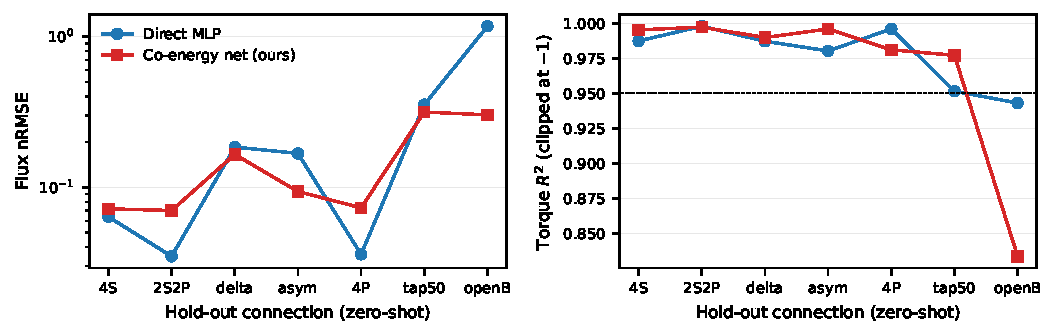
\includegraphics[width=\linewidth]{figs/fig_benchmark.pdf}
\caption{Zero-shot benchmark across the seven hold-out connections
(base variant). Left: flux nRMSE (log scale); right: torque $R^2$.
Tier-1 hold-outs transfer at in-distribution accuracy; tier-3 hold-outs
require pattern coverage; the monotone vector field fails everywhere.}
\label{fig:benchmark}
\end{figure}

\begin{figure}[t]
\centering
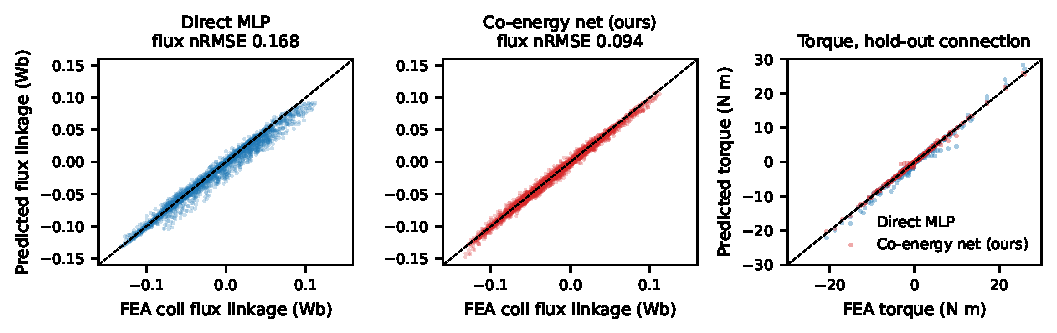
\includegraphics[width=\linewidth]{figs/fig_parity.pdf}
\caption{Hold-out connection \emph{asym}: predicted vs FE coil flux
linkages (left: direct MLP; centre: co-energy net) and torque (right).}
\label{fig:parity}
\end{figure}

Table~\ref{tab:main} and Fig.~\ref{fig:benchmark} report all hold-outs;
Fig.~\ref{fig:parity} shows parity plots for the hardest LOCO hold-out.
As a quantitative anchor for
Prop.~\ref{prop:bound}, we compute for each hold-out the mean min-distance
$\bar d$ of its test current vectors (normalised by the 60\,A scale) to
the sampled training support: 4P $0.036$, 2S2P $0.055$, asym $0.206$,
delta $0.240$, 4S $0.263$, openB $0.288$, tap50 $0.536$. Across the seven
hold-outs the rank correlation with the zero-shot flux error is
$\rho=0.82$ ($p=0.02$). The correlation is meaningful but not perfect,
and the misalignment is informative: openB sits at a modest $\bar d$ yet
fails hardest ($1.38$), because its sign-flipped phase pairs are
\emph{close} in Euclidean distance to the training support while lying in
a direction the support barely samples---an unweighted distance metric
cannot see support density or direction. The 4S hold-out supplies the
opposite counterexample: its distance is high ($0.263$) while its flux error
is low ($0.093$). We therefore use $\bar d$ only as a coarse risk indicator;
neither a large nor a small value justifies accepting or rejecting a
connection. Four observations.

\textbf{(1) In-support transfer is essentially free.} For tier-1 hold-outs
(2S2P, 4P) the shared model reaches flux nRMSE $0.02$--$0.05$ and torque
$R^2\ge0.96$, i.e.\ in-distribution accuracy: their current subspaces lie
inside the training support ($\bar d<0.06$, Prop.~\ref{prop:bound}), so
the connection adds no error of its own. Notably, 4P was
\emph{never seen}---it is a rescaled 4S, and the model treats it as such.

\textbf{(2) Without pattern coverage, tier-3 collapses to chance.} When
trained on the standard connections only (``no-random''), every model
predicts flux on asym at nRMSE $\approx1.0$---no better than predicting
the mean. (The flux channel collapses; the torque channel partially
survives at $R^2\approx0.95$ because the dominant average-torque trend is
recoverable from the rotor-angle features alone---a caution against
judging such models by torque $R^2$ only.) This is the single most
important negative control in the benchmark: connection labels are
worthless; current-space coverage is everything.

\textbf{(3) Magnitude patterns rescue unbalance.} Adding 48 magnitude-random
groups brings asym to $0.11$ (MLP) and $0.13$--$0.16$ (co-energy nets);
MLP torque $R^2$ reaches $0.85$--$0.90$ (co-energy $0.69$).

\textbf{(4) Phase patterns rescue open-phase.} Magnitude patterns leave
openB at $1.38$; 24 phase-random groups bring it to $0.066$
(\S\ref{sec:results:phase})---the second design principle.

\begin{table}[t]
\centering\small
\caption{Zero-shot benchmark, flux nRMSE / torque $R^2$. Training variants:
``base'' = three standard connections (all four for EXT rows) + 48
magnitude-random groups + PM data; ``withz'' = base + the 24 zero-support
pattern groups; ``no random'' = standard connections + PM data only.
LOCO rows hold out one standard connection; EXT rows (4P, tap50, openB) hold
out connections never seen at all. Best per row in bold.}
\label{tab:main}
\resizebox{\linewidth}{!}{%
\begin{tabular}{llccc}
\toprule
Tier & Hold-out & Direct MLP & Co-energy (ours) & Monotone VF \\
\midrule
1 & 4S (LOCO)      & \textbf{0.093}/\textbf{0.930} & 0.132/0.658 & 0.414/$-0.68$ \\
1 & 2S2P (LOCO)    & \textbf{0.041}/\textbf{0.994} & 0.090/0.961 & 0.382/$-0.53$ \\
1 & 4P (EXT)       & \textbf{0.047}/\textbf{0.960} & 0.094/0.838 & 0.409/$-8.2$ \\
2 & delta (LOCO)   & 0.356/\textbf{0.840} & \textbf{0.201}/$-0.05$ & 0.424/$-2.0$ \\
3 & asym (LOCO)    & \textbf{0.113}/\textbf{0.897} & 0.152/0.689 & 0.495/$-1.7$ \\
3 & tap50 (EXT)    & 0.427/0.696 & \textbf{0.363}/\textbf{0.811}$^\dagger$ & 0.479/$-0.14$ \\
3 & openB (EXT)    & 1.379/0.288 & \textbf{0.472}/$-18.5$ & 0.563/$-5.6$ \\
\midrule
\multicolumn{2}{l}{asym, no random patterns} & 1.002/0.949 & 1.000/0.397 & 0.990/$-0.20$ \\
\multicolumn{2}{l}{asym, per-connection MLP (4S only)} & 1.002/0.930 & --- & --- \\
\multicolumn{2}{l}{asym, linear ridge (reciprocity-structured)} & \multicolumn{3}{c}{0.652} \\
\bottomrule
\multicolumn{5}{l}{\footnotesize $^\dagger$with zero-support patterns included
(``withz'' variant); see \S\ref{sec:results:phase}.} \\
\end{tabular}
}
\end{table}

\subsection{What kind of coverage matters}
\label{sec:results:phase}

\begin{figure}[t]
\centering
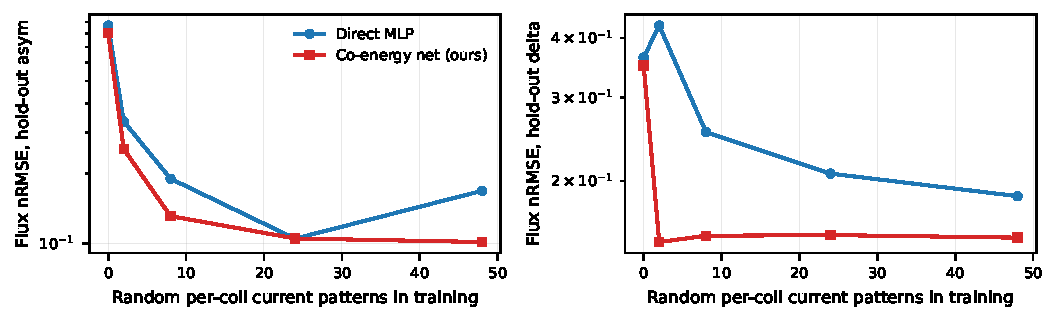
\includegraphics[width=\linewidth]{figs/fig_scaling.pdf}
\caption{Coverage scaling of magnitude-random patterns on the two
hardest standard hold-outs. asym improves monotonically with pattern
count; delta is insensitive to it---its requirement is phase coverage
(Table~\ref{tab:phase}).}
\label{fig:scaling}
\end{figure}

Fig.~\ref{fig:scaling} shows the coverage-scaling curves;
Table~\ref{tab:phase} isolates the effect, and it is sharper than
anticipated: the two pattern families rescue \emph{disjoint} connection
classes. Magnitude patterns bring tap50 from $1.86$ to $0.43$ (they sample
non-uniform per-coil amplitudes, including small ones) but leave openB at
$1.39$ (open-phase operation drives sign-flipped phase pairs that
multiplicative perturbations of a balanced base never generate). Phase-random
patterns do the opposite: openB drops to $0.066$ ($R^2=0.99$) and delta from
$0.27$ to $0.072$ (delta is itself a phase-recombination), while tap50
degrades to $2.1$ in that pool alone (phase-random patterns keep all coils
energised). With both families in the pool (a quarter of the magnitude
family's FE cost added on top), each hold-out is served by the family it
needs: openB $0.09$, delta $0.08$, tap50 $0.43$ (via either family's best).
On delta, moreover, scaling the
\emph{magnitude} family from 0 to 48 groups leaves the error essentially
unchanged ($0.27$ at zero groups, $0.26$ at 24, $0.36$ at 48)
($0.27\to0.36$), while a quarter-sized phase family reaches $0.07$: coverage
\emph{kind} dominates coverage \emph{amount}. This is consistent with the
qualitative implication of Prop.~\ref{prop:bound}, although the bound itself
is not tight in Euclidean distance.

\begin{table}[t]
\centering\small
\caption{Coverage-kind ablation (flux nRMSE / torque $R^2$). Hold-outs:
openB = phase-B open circuit, tap50 = half-winding series tap, delta =
star--delta recombination. Magnitude patterns (48 groups, 4{,}608 FE
samples) and phase patterns (24 groups, 1{,}152 samples) rescue
\emph{different} hold-out connections; the union covers all.}
\label{tab:phase}
\begin{tabular}{lccc}
\toprule
Training pool & openB & tap50 & delta \\
\midrule
standard only            & 1.83/$-0.62$ & 1.86/0.41 & 0.27/0.84 \\
+ magnitude (48 groups)  & 1.38/\phantom{$-$}0.29 & \textbf{0.43}/0.70 & 0.36/0.84 \\
+ phase (24 groups)      & \textbf{0.07}/\textbf{0.99} & 2.11/$-0.01$ & \textbf{0.07}/\textbf{0.99} \\
+ both                   & 0.09/0.97 & 0.43/\textbf{0.73} & 0.08/0.98 \\
\bottomrule
\end{tabular}
\end{table}

\subsection{Physical consistency}
\label{sec:results:jacobian}

\begin{figure}[t]
\centering
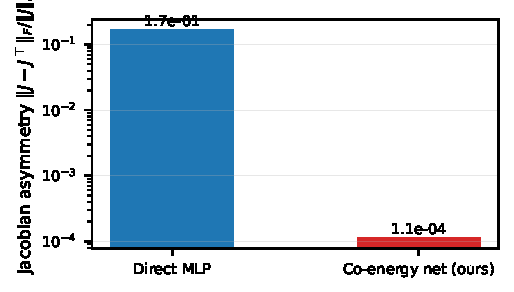
\includegraphics[width=0.6\linewidth]{figs/fig_jacobian.pdf}
\caption{Flux-Jacobian reciprocity residual on held-out operating points
(log scale): the co-energy network violates reciprocity nearly three orders of
magnitude less than the direct MLP.}
\label{fig:jacobian}
\end{figure}

Table~\ref{tab:jacobian} and Fig.~\ref{fig:jacobian} evaluate the flux Jacobian
$\partial\hat{\psic}/\partial\ic$ by central differences on 24 held-out
operating points. The co-energy network violates reciprocity by
$4.6\times10^{-4}$---nearly three orders of magnitude below the direct MLP's
$0.22$---and keeps a positive-definite symmetric part (min eigenvalue
$0.36>0$, physically admissible incremental inductances). The monotone
vector field is exactly symmetric by construction ($1.6\times10^{-5}$) but,
as the next section shows, fits nothing.

\begin{table}[t]
\centering\small
\caption{Jacobian reciprocity and positive-definiteness on held-out points
(asym).}
\label{tab:jacobian}
\begin{tabular}{lccc}
\toprule
Model & $\|J-J^{\!\top}\|_F/\|J\|_F$ & min eig$(\frac{J+J^\top}{2})$ \\
\midrule
Direct MLP & $0.221$ (max $0.363$) & $0.340$ \\
Co-energy (ours) & $4.6\times10^{-4}$ (max $2.2\times10^{-3}$) & $0.359$ \\
Monotone VF & $1.6\times10^{-5}$ & $0.278$ \\
\bottomrule
\end{tabular}
\end{table}

\subsection{Negative result: monotonicity is the wrong structure}
\label{sec:results:neg}

The monotone vector field enforces joint convexity of the underlying scalar
in $(\ic,\phi)$. The true co-energy is approximately convex in $\ic$ alone at
fixed $\theta$, but its $\theta$-dependence through the PM field and slotting
makes the joint Hessian indefinite; the architecture can therefore only fit a
compromise, and lands at flux nRMSE $0.28$--$0.99$ and strongly negative
torque $R^2$ at every tier, including in-support (4S LOCO $0.41$,
single-connection-trained variant $0.48$), so the failure is not an
artefact of cross-connection sharing. Stronger
training (2$\times$ epochs, $3\times$ learning rate) does not
close the gap either: the failure is structural rather than one of
optimisation.
The lesson for structural design in magnetic ML: \emph{enforce the physical
symmetries the PDE actually has (reciprocity, potential structure), not
convenient convexity properties it does not have}. Scalar co-energy
parameterisations get the former for free.

\subsection{Data efficiency and coverage scaling}

\begin{figure}[t]
\centering
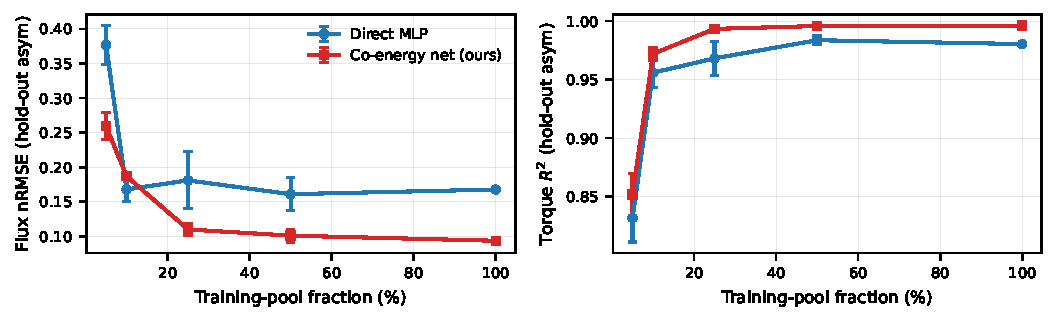
\includegraphics[width=\linewidth]{figs/fig_curves.pdf}
\caption{Data-efficiency learning curves on the hold-out connection
(three seeds): flux nRMSE (left) and torque $R^2$ (right) vs fraction of
the training pool.}
\label{fig:curves}
\end{figure}

Scaling the magnitude-pattern family on the unbalanced hold-out (asym, MLP):
$0$ groups $1.00$, $2$ groups $0.51$, $8$ groups $0.22$, $24$ groups $0.16$,
$48$ groups $0.11$---a clean coverage curve that saturates near 24--48
groups, i.e.\ a few thousand FE samples. On delta the same family leaves
the error essentially unchanged ($0.27$ at zero groups, $0.26$ at 24,
$0.36$ at 48), while the
quarter-sized phase family reaches $0.07$ (\S\ref{sec:results:phase}), which
is the coverage-kind argument in its purest form.

Fig.~\ref{fig:curves} shows subsampling of the full training pool (three
seeds, hold-out asym): the
MLP reaching nRMSE $0.22$ with only $10\,\%$ of the data (497 samples) and
$0.17$ at $25\,\%$; the co-energy net needs $\sim$25\,\% of the pool to
reach its plateau ($0.15$--$0.19$) and its torque channel degrades more
sharply in the extreme low-data regime ($5\,\%$: $R^2<0$), consistent with
its gradient-based outputs needing more support to anchor the residual head.
The practical reading: with adequate pattern coverage, a few hundred FE samples
already yield usable zero-shot flux models; the structured head is worth its
consistency guarantee once at least a quarter of the pool is available.

\subsection{Cross-machine replication}
\label{sec:results:machine2}

To test whether the two coverage principles are artefacts of one machine,
we repeated the core ablations on a second machine with the same solver
family: a 6-slot/4-pole SPM (different slot count, winding factor,
inductance matrix and harmonic content; 3{,}084 FE samples in the same
dataset families). With a direct MLP and the identical protocol, the
pattern repeats: the half-winding tap hold-out improves with
\emph{magnitude}-random patterns (flux nRMSE $0.62\!\to\!0.30$; phase
patterns alone leave it at $0.65$), while the open-phase hold-out is
rescued by \emph{phase}-random patterns ($1.11\!\to\!0.08$; magnitude
patterns alone leave it at $1.08$). The union pool again serves both
($0.30$ and $0.065$). Which family a connection needs tracks the geometry
of its current vectors, not the machine---as the coverage argument
requires.

\begin{table}[t]
\centering\small
\caption{Cross-machine replication on the 6-slot/4-pole SPM. Entries are
flux nRMSE / torque $R^2$ for the direct MLP. The co-energy network was not
re-trained for this replication, so the table tests the two sampling
principles rather than architecture ranking.}
\label{tab:machine2}
\begin{tabular}{lcccc}
\toprule
Hold-out & Standard & + magnitude & + phase & + both \\
\midrule
tap50 & 0.620/0.753 & \textbf{0.296/0.821} & 0.648/0.788 & 0.304/\textbf{0.881} \\
openB & 1.110/0.753 & 1.079/0.783 & 0.082/\textbf{0.997} & \textbf{0.065}/0.992 \\
\bottomrule
\end{tabular}
\end{table}

\section{Drive-cycle co-design case study}
\label{sec:drive}

\subsection{From surrogate to system losses}

Unless stated otherwise, the drive-cycle study uses the direct-MLP
surrogate as the reference model: it is the most accurate of
\S\ref{sec:results} on the connections involved, and the co-energy
surrogate is used below as an independent cross-check that brackets the
conclusions. The surrogate is queried in a synchronous-rotating frame. For a mode $m$
with connection matrix $\Cmat_m$, line-current amplitude $I$ and current
angle $\gamma$, the phase currents rotate as
$i_p(t)=I[\cos(2\theta+\gamma),\cos(2\theta+\gamma-\tfrac{2\pi}{3}),
\cos(2\theta+\gamma+\tfrac{2\pi}{3})]$. Average torque, copper loss, the
iron-loss proxy and the port voltage then follow from one electrical
period of surrogate evaluations ($12\times$ torque grid, $72\times$
voltage grid), giving loss maps $P_{\text{loss}}^{m}(T,\omega)$ and
voltage envelopes $V^{m}(I,\omega)\le V_{dc}/\sqrt{3}$ per mode in under
a second on GPU. The loss model comprises exact copper loss
$\sum_c i_c^2R_c$ from the coil currents; inverter conduction and
switching from declared device parameters
($V_{CE0}=0$\,V, $r_{CE}=0.5$\,m$\Omega$, $E_{sw}=0.1$\,mJ per period at
10\,kHz, an idealised linear 400-V SiC stage); a Bertotti-type
\cite{Bertotti1998} iron-loss proxy on the
AC coil-flux amplitude
(coefficients stated in the released configuration, $\pm2\times$ swept);
and a changeover energy $E_{sw}^{c}$ per reconfiguration event
(5\,mJ--100\,J swept). The vehicle is a \SI{540}{kg} light EV with four
identical wheel motors, each supplying one quarter of the wheel torque
through gear 20 (wheel \SI{0.25}{m}, $C_dA=0.50$\,m$^2$, 400\,V bus,
50\,\% slot fill). This sizing gives the fixed 4P baseline an $81.8\,\%$
traction efficiency, and the cycle is the
official WLTC class-1 trace \cite{UNECE2015} (JRC data,
checksum-verified). The trace spans
the machine's full mode space: 4S is efficient at low load but cannot cover
the full demand envelope; 2S2P, delta and 4P complete the cycle. At matched
sizing, fixed delta is the best fixed connection at $85.1\,\%$ traction
efficiency, so the case tests whether scheduling brings any incremental
value rather than assuming that reconfiguration must win.

\subsection{Scheduling formulation}

With per-step mode-conditioned optimal operating points, mode selection is a
shortest-path problem over a mode graph with dwell constraints. We solve it
by dynamic programming on the state (mode, steps-since-last-switch) with
minimum dwell $D=10$\,s, comparing: \textbf{fixed-delta} (the best fully
feasible fixed connection), \textbf{fixed-4P} (the conservative
single-inverter baseline),
\textbf{2-mode rule} (4S/4P at a swept speed threshold, the practice of
\cite{Shin2024WEVJ}), \textbf{pointwise greedy}, and \textbf{DP}.

\subsection{Results}

\begin{figure}[t]
\centering
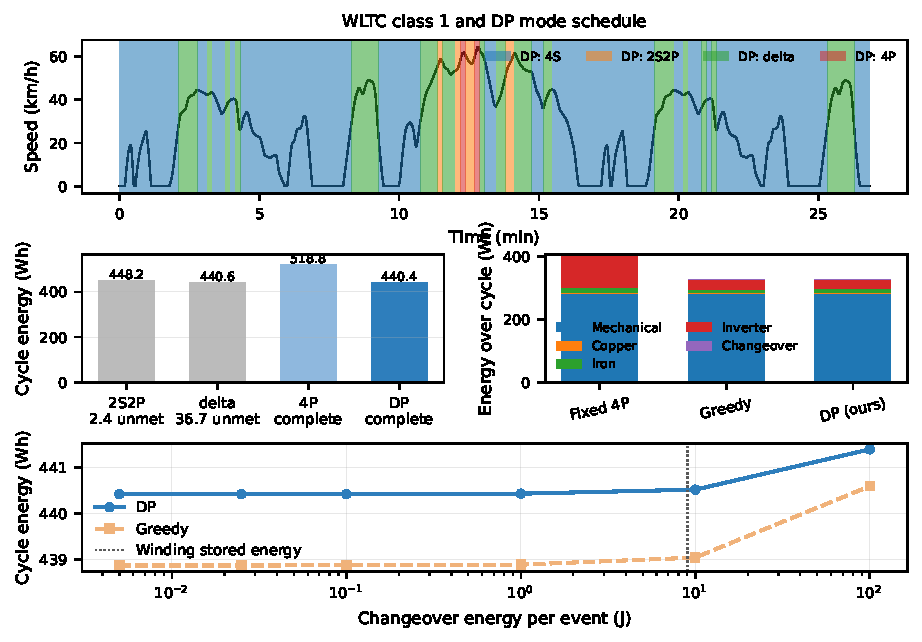
\includegraphics[width=\linewidth]{figs/fig_drive.pdf}
\caption{Drive-cycle case study. Top: WLTC class-1 speed trace and the DP
mode schedule (colour band). Middle-left: fixed-connection and DP cycle
energy; incomplete trajectories are marked by their unmet torque integral.
Middle-right: loss decomposition for completed trajectories. Bottom:
sensitivity of cycle energy to the changeover energy, swept from 5\,mJ to
100\,J.}
\label{fig:drive}
\end{figure}

Table~\ref{tab:drive} and Fig.~\ref{fig:drive} summarise the case study.

\textbf{Reconfiguration is valuable only in the constrained-voltage
regime.} At 400\,V, fixed 4P is the only fully feasible fixed connection:
it consumes $472.7$\,Wh ($41.36$\,Wh/km) at $81.8\,\%$ traction efficiency.
The DP schedule uses $458.3$\,Wh ($40.10$\,Wh/km) at $84.7\,\%$ efficiency
with 54 changeover events (4.7 per km), a $3.1\,\%$ saving. Fixed 2S2P and
delta would consume less energy ($371.9$ and $387.3$\,Wh), but leave $4.05$
and $8.87\,\%$ of the torque integral unmet, with peak per-motor gaps of
$0.53$ and $0.64$\,N\,m. Fixed 4S is substantially worse ($34.7\,\%$
unmet). The voltage sweep identifies the boundary: at 700\,V and above,
fixed delta becomes fully feasible and the DP gain collapses to
$0.4$--$0.6\,\%$.

The exact gain remains model-sensitive: the co-energy surrogate evaluates
the same 400-V DP schedule at $438.1$\,Wh and fixed 4P at $473.6$\,Wh,
implying a $7.5\,\%$ saving. The direct MLP and co-energy estimates therefore
disagree by $4.4$ percentage points. The composition of the 4P-to-DP
difference is partly inverter-driven: inverter loss falls from $21.0$ to
$3.0$\,Wh, iron loss from $37.0$ to $34.4$\,Wh, while copper loss rises
from $19.0$ to $20.7$\,Wh. The magnetic surrogate supplies the operating
points, but the reported saving cannot be attributed to magnetic accuracy
alone.

\textbf{Optimal scheduling matches the pointwise oracle at substantially
lower switching burden.} The per-point greedy oracle gives $457.64$\,Wh
with 139 switches; DP gives $458.25$\,Wh with 54 switches. The energy
difference is $0.62$\,Wh, while DP avoids 85 changeover events. A classical
two-mode speed-threshold rule uses only $195.9$\,Wh on its nominal path but
leaves $30.7\,\%$ of the torque integral unmet (peak gap $1.03$\,N\,m per
motor); that energy is not comparable. This is the
failure mode that motivates schedule-level optimisation over rule-based
switching.

\textbf{The saving is robust across physically meaningful changeover
energies.} The default per-event cost ($25$\,mJ) sits far below the
physics: the winding stores $\approx$\,9\,J of magnetic energy at typical
commutation currents, which any real changeover device must dissipate or
commutate. Sweeping the per-event energy over four orders of
magnitude---$5$\,mJ to $100$\,J---leaves the DP schedule identical (54
events at every value) and costs at most $1.5$\,Wh at the
extreme end; even at $100$\,J per event, ten times the stored magnetic
energy, the schedule still completes the cycle. Scaling the iron-loss
coefficients by $0.5\times$ and $2\times$ keeps the DP-vs-4P difference
between $2.9\,\%$ and $3.1\,\%$. These sweeps establish robustness of the
\emph{conditional} scheduling benefit.

\textbf{Device rescaling and surrogate uncertainty.} Each motor uses one
inverter for all modes, which flatters low-current modes (4S at a quarter of
4P's line current). Re-running with current-class-matched
device parameters ($r_{CE}$ halved, $V_{CE0}$ $+10\,\%$) changes the
DP-vs-4P difference from $3.1\,\%$ to $1.9\,\%$. Re-evaluating the same
schedule with the independent co-energy surrogate gives $7.5\,\%$, not a
small perturbation. This model-to-model spread is the dominant uncertainty.
The
mode histogram is
physically interpretable: 4S dominates low-speed urban segments
(763\,s), delta carries mid-speed cruising (429\,s), 2S2P contributes
251\,s, and 4P appears in the 168\,s highest-demand phase.

\subsection{Zero-shot modes and connection screening}
\label{sec:results:zeroshot}

The drive study above schedules four connections that all appear in the
training pools. The point of the connection-invariant formulation,
however, is that a candidate $\Cmat$ can be queried without new FE data or
retraining, subject to coverage. Two experiments exercise this.

\textbf{A zero-shot candidate exposes the limit of screening.} We add
tap50---never present in the drive surrogate's training pool in any
form---as a fifth switchable mode. The surrogate assigns it zero seconds,
which would suggest that 2S2P/delta dominate it on the cycle. The
independent FEMM trajectory check does not support that action: the
zero-shot direct MLP gives torque correlation $0.66$ but raw $R^2=-0.38$
at 36 FEMM points; the co-energy variant improves correlation to $0.73$
but its raw $R^2$ is only $0.26$. The never-trained 3S1P connection behaves
differently: the same zero-support MLP reaches torque correlation $0.79$
and $R^2=0.58$, so the boundary is coverage rather than an inability to
transfer at all. The
tap50 flux trend is informative enough to generate
a hypothesis, but the torque channel is not reliable enough to reject the
connection. We report this as a negative result for automatic zero-shot
screening.

\textbf{Connection screening at design time.} Table~\ref{tab:screen}
evaluates eight candidate connections (including three tap ratios and an
unbalanced 3S1P split, all zero-shot for the tap/3S1P entries) as fixed
connections over the same cycle. It is a screening experiment, not a
validated ranking: the tap50 FEMM check above shows that the torque channel
can fail on an unseen synchronous path. The table is useful for forming
FE validation priorities in minutes, but a candidate that survives this
screen still requires targeted FE checks before a design decision.

\begin{table}[t]
\centering\small
\caption{Exploratory zero-shot screening: fixed-connection cycle energy and
unmet torque integral (WLTC class 1). Entries marked $^\ast$ are absent from
the drive training pool. The tap50 FEMM check shows that these surrogate
rankings require targeted FE validation before use as design decisions.}
\label{tab:screen}
\begin{tabular}{lcc}
\toprule
Connection & Energy (Wh) & Unmet torque (N\,m\,s) \\
\midrule
4S        & (146.8) & 876.8 \\
2S2P      & (371.9) & 102.2 \\
delta     & (387.3) & 224.1 \\
4P        & 472.7 & 0.0 \\
3S1P$^\ast$ & (132.0) & 793.4 \\
tap75$^\ast$ & (108.0) & 1{,}117.3 \\
tap50$^\ast$ & (93.1) & 748.9 \\
tap25$^\ast$ & (118.2) & 1{,}508.4 \\
\bottomrule
\end{tabular}
\end{table}

\begin{table}[t]
\centering\small
\caption{Drive-cycle case study: WLTC class-1, 540-kg four-wheel-drive
light EV with four identical motors, 400-V SiC drive, 11.43\,km, all losses
counted, minimum dwell 10\,s. Energy in parentheses belongs to an incomplete
trajectory and is descriptive only; comparisons are shown only for
completed trajectories.}
\label{tab:drive}
\resizebox{\linewidth}{!}{%
\begin{tabular}{lcccccc}
\toprule
Strategy & Complete & Energy (Wh) & Wh/km & vs DP & Switches &
Unmet torque (N\,m\,s) \\
\midrule
Fixed 4S         & no  & (146.8) & ---    & ---      & 0  & 876.8 (34.72\%) \\
Fixed 2S2P       & no  & (371.9) & ---    & ---      & 0  & 102.2 (4.05\%) \\
Fixed delta      & no  & (387.3) & ---    & ---      & 0  & 224.1 (8.87\%) \\
Fixed 4P         & yes & 472.7   & 41.36  & +3.15\,\% & 0  & 0 \\
2-mode rule      & no  & (195.9) & ---    & ---      & 5  & 775.4 (30.70\%) \\
Pointwise greedy & yes & 457.6   & 40.05  & $-0.13\,\%$ & 139 & 0 \\
DP (ours)        & yes & 458.3   & 40.10  & 0        & \textbf{54} & 0 \\
\bottomrule
\end{tabular}
}
\end{table}

\section{Discussion and limitations}
\label{sec:discussion}

\textbf{Design principles for connection benchmarks.} The two coverage
principles (magnitude families for unbalance, phase families for
phase-recombining connections) are motivated by
Prop.~\ref{prop:bound}. We expect them to carry over to other
machines: pattern families should be chosen by the span of the target
connections' current vectors, not by sample count. Multi-phase and fault
reconfiguration studies are the natural next testbeds, where the
``phase'' family is the default recommendation.

\textbf{What structure buys.} On the \emph{flux} channel the structured
co-energy network improves on the MLP for tap50 and openB but not for asym,
and concedes accuracy on tier-1 hold-outs, in exchange for exact potential
structure. Its \emph{torque} channel, however, is
consistently weaker ($R^2$ as low as $-18.5$ on openB, $-0.05$ on delta):
differentiating a learned scalar amplifies residual error, so
torque-critical applications should either up-weight the torque loss
further or accept the MLP's pointwise torque. In downstream use where
consistency matters (optimisation, control, port-level circuit solving)
the structured model can never produce non-conservative operating points;
the Jacobian evidence (Table~\ref{tab:jacobian}) quantifies the
difference. Our benchmark makes this trade-off explicit rather than
hiding it.

\textbf{Limitations.} (i)~2-D magnetostatics with a research-grade solver;
the fine-mesh check (Table~\ref{tab:feacheck}) bounds discretisation
uncertainty at a mean $10\,\%$ (max $30\,\%$) on flux and $13\,\%$ median on torque.
This is of the same order as the reported model errors ($0.04$--$0.4$
nRMSE), so \emph{absolute} accuracies should be read as accuracy relative
to this discretisation. The FEMM cross-check corroborates matrix and waveform
trends but also shows metric-dependent discrepancies: a residual $1.13\times$
inductance normalisation factor with a $2.1\,\%$ fine-mesh shape residual,
$1.2\,\%$ for saturated torque, $38.3\,\%$ for the coverage-trained tap50
flux shape, and $84.7$--$98.2\,\%$ for its torque shape. It
therefore does not establish absolute accuracy or a reliable zero-shot
torque screen (Table~\ref{tab:femmcheck}). (ii)~End effects, temperature, mechanical and changeover
transients are excluded; the changeover circuit enters through a per-event
energy, swept over four orders of magnitude ($5$\,mJ--$100$\,J).
(iii)~The drive-cycle study is a
simulation case study on a laboratory-scale machine; absolute savings
percentages are machine- and vehicle-specific, and we make no homologation
claims. (iv)~Iron loss is a Bertotti proxy calibrated to the assumed steel
curve, not measured. (v)~External validity: the quantitative benchmark
and the drive-cycle case study derive from a single machine; the two
coverage \emph{principles}, however, are replicated on a second machine
(\S\ref{sec:results:machine2}). All ground truth remains simulation-only,
and no measurement validation was performed. A commercial FE cross-check is
reported in Table~\ref{tab:femmcheck}; it exposes both
discretisation/model-form differences and a zero-shot torque failure on an
untrained tap connection. Replication on a measured machine remains required
before the design principles can be treated as general.

\section{Conclusion}
\label{sec:conclusion}

A winding connection is a linear constraint, not a new machine. Encoding
that fact into the learning problem yields one surrogate queryable across
winding connections, coverage-dependent zero-shot transfer, and exact physical
consistency from a scalar co-energy head. It also yields a
drive-cycle co-design loop that prices reconfiguration with full loss
accounting---changeover energy, dwell constraints and system losses. On
the 400-V WLTC class-1 case study, the optimal schedule uses $458.3$\,Wh
and saves $3.1\,\%$ against the only fully feasible fixed connection. The
independent co-energy surrogate estimates $7.5\,\%$, so the magnitude is
not established. Raising the bus to 700\,V makes fixed delta feasible and
reduces the gain below $0.6\,\%$. Reconfiguration should therefore be
justified by a specific voltage/current constraint, not assumed to improve
efficiency. The benchmark
and its two data-design
principles are, we believe, the most durable contributions: they tell the
next study, whatever its machine, what data to collect and why. Future
work will address geometry-parametric co-energy operators (design-space
generalisation), thermal coupling, and hardware validation of the
scheduling layer on a changeover test rig.

\section*{Reproducibility}

All FE data (23{,}000+ samples across the benchmark and drive-cycle pools),
the solver, the training and evaluation
code, trained checkpoints, benchmark splits, the official WLTC class-1
trace preprocessing, the second-machine replication scripts, the FEMM
cross-check and the 36-point unseen-connection tests, and
one-command figure scripts are released at
\todonum{[repository URL on acceptance]}.

\bibliographystyle{elsarticle-num}
\begin{thebibliography}{23}

\bibitem{Best2025Access}
D.~Best, P.~Asef, C.~Vagg, Reconfigurable electric machine windings: A
technology review, IEEE Access 13 (2025) 140187--140202.

\bibitem{Shin2024WEVJ}
M.~Shin, K.~Cho, J.-Y. Lee, A study on series--parallel winding changeover
circuit and control method for expanding the operating range of an 80-kW-class
EV traction motor, World Electric Vehicle Journal 15~(11) (2024) 501.

\bibitem{TMAG2012Changeover}
Z.~Wu, Z.~Q. Zhu, Winding changeover permanent-magnet generators for
renewable energy applications, IEEE Transactions on Magnetics 48~(11) (2012)
4129--4132.

\bibitem{Guo2026Electronics}
X.~Guo et~al., Seamless winding changeover for series--parallel
reconfigurable PMSM drives via zero-voltage-vector deadbeat predictive
current control, Electronics 15~(20) (2026) 3120.

\bibitem{TPEL2026Seamless}
Fast seamless series--parallel winding transition for extended-speed PMSM
drives, IEEE Transactions on Power Electronics (2026).
doi:10.1109/TPEL.2026.3697314.

\bibitem{JESTPE2026Seamless}
Zero-voltage-vector interval-based seamless winding reconfiguration,
IEEE Journal of Emerging and Selected Topics in Power Electronics (2026).
doi:10.1109/JESTPE.2026.3687988.

\bibitem{Energies2026Ich}
S.~Kallur-Krishnamoorthy et~al., Normalised characteristic current criteria
for star/delta and series--parallel reconfigurable windings, Energies 19
(2026) 4849.

\bibitem{Access2020ANNReview}
Artificial-neural-network torque surrogate models for electrical machines: a
review, IEEE Access 8 (2020) 211935--211952.
doi:10.1109/ACCESS.2020.3042834.

\bibitem{TEC2025PINN}
Physics-informed neural networks for parametric modelling of permanent
magnet synchronous machines, IEEE Transactions on Energy Conversion (2025).
doi:10.1109/TEC.2025.3597814.

\bibitem{Arxiv2024POD}
Proper orthogonal decomposition and support-vector-regression fast surrogate
modelling of electrical machines, arXiv:2406.18990 (2024).

\bibitem{DETC2025FNO}
Fourier neural operator acceleration of electromagnetic FE simulation of
electric machines, ASME IDETC/CIE (2025). doi:10.1115/DETC2025-168594.

\bibitem{Li2026GradNet}
Li et~al., Gradient networks for universal magnetic modelling of synchronous
machines, arXiv:2602.14947 (2026).

\bibitem{TIA2024MechChangeover}
Induction motor drive system with novel mechanical winding changeover
device, IEEE Transactions on Industry Applications (2024).
doi:10.1109/TIA.2024.3464567.

\bibitem{IPEC2014}
A wide speed range high efficiency EV drive system using winding changeover
technique, IPEC-Hiroshima (2014). doi:10.1109/IPEC.2014.6869844.

\bibitem{Cha2024Math}
S.-H. Cha et~al., Open-end winding with series--parallel mode switching for
energy-efficient EV drives, Mathematics 12~(22) (2024) 3415.

\bibitem{TIE2026Tap}
Three-speed tapped IPMSM drive, IEEE Transactions on Industrial Electronics
(2026). doi:10.1109/TIE.2025.3591670.

\bibitem{TTE2025SRM}
Reconfigurable three-switch SRM windings, IEEE Transactions on
Transportation Electrification (2025). doi:10.1109/TTE.2024.3416151.

\bibitem{Raissi2019PINN}
M.~Raissi, P.~Perdikaris, G.~E. Karniadakis, Physics-informed neural
networks, Journal of Computational Physics 378 (2019) 686--707.

\bibitem{Li2021FNO}
Z.~Li et~al., Fourier neural operator for parametric partial differential
equations, ICLR (2021).

\bibitem{Amos2017ICNN}
B.~Amos, L.~Xu, J.~Z. Kolter, Input convex neural networks, ICML (2017)
146--166.

\bibitem{Bertotti1998}
G.~Bertotti, Hysteresis in Magnetism, Academic Press, 1998.

\bibitem{UNECE2015}
UNECE, Global technical regulation No.~15 (WLTP), ECE/TRANS/2015 (2015).

\bibitem{RSER2025}
Machine-learning-assisted multi-objective optimisation of electrical
machines: a review, Renewable and Sustainable Energy Reviews (2025).
doi:10.1016/j.rser.2025.115609.

\end{thebibliography}

\end{document}
